\documentclass[12pt]{article}

\usepackage[T1]{fontenc}
\usepackage[a4paper, margin=1.5cm]{geometry}
\usepackage[colorlinks, urlcolor=blue, citecolor=red]{hyperref}
\usepackage[utf8]{inputenc}
\usepackage{amsmath, amsfonts, enumitem, parskip, tikz}
\usetikzlibrary{arrows,automata}

\newcommand{\e}{\varepsilon}

\begin{document}

\textsc{Graduate Program in Computer Science,
Universidade Federal de Santa Catarina} \\
\textsc{INE410113 (Theory of Computation)}

\textsc{Converting NFAs to regular expressions
with the Brzozowski algebraic method} \\
\textsc{Gustavo Zambonin}

An arguably simple method to convert non-deterministic finite automata (NFA) to
regular expressions is due to Brzozowski~\cite{Brzozowski:article:1964:oct}. It
expresses the automaton as a system of equations, in which each equation
describes the language accepted by a particular state of the automaton. The
objective is to solve the system until only a single equation is left,
featuring a closed form regular expression.

Consider a NFA $A = (Q, \Sigma, \delta, q_0, F)$ free of $\e$-transitions, and
in this context, operations of union ($\cup$), concatenation ($\cdot$) and
Kleene star ($^*$). Associativity and distributivity of union and
concatenation, and commutativity of union are desired properties for this
method to work. Furthermore, we will observe shortly that the systems generated
may only be solved if we also take into account the lemma below.

\emph{Arden's lemma~\cite{Arden:inproc:1961:oct}.} Let $L, U, V \subseteq
\Sigma^*$ be regular languages with $\e \not\in U$. Then,
\begin{equation}\label{eq:arden}
  L = UL \cup V \Leftrightarrow L = U^*V.
\end{equation}
The description for the method is as follows. For every state $q_i\in Q$,
create the equation
\begin{equation}\label{eq:brzo}
  Q_i = \bigcup\limits_{q_i \overset{a}{\to} q_j} aQ_j \cup
  \begin{cases}
      \{\e\},       & q_i \in F \\
      \emptyset,    & q_i \not\in F,
  \end{cases}
\end{equation}
and solve the system for $Q_0$, using the properties of operations listed
above, as well as Eq.~\ref{eq:arden}.

\emph{Example.} Consider the regular language $\mathcal{L} = \{w \mid w \in
\Sigma^* \land \texttt{110110} \text{ is not a substring of } w\}$.

We will first need to build an automaton which accepts this language. Note that
we can build $\overline{\mathcal{L}}$, that is, the language that accepts every
string which contains \texttt{110110}, and then invert accepting and
non-accepting states. This is allowed, since regular languages are closed under
complement. We present the output of this rationale below.

\begin{figure}[htbp]
  \centering
  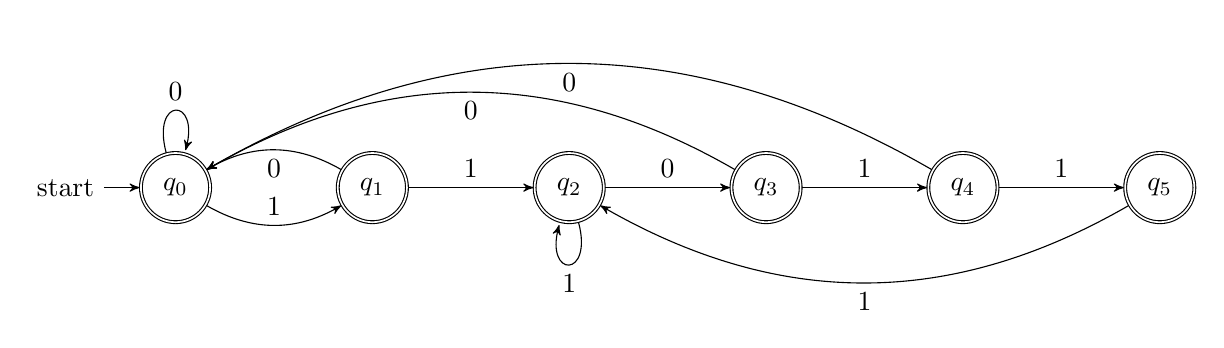
\begin{tikzpicture}[->,>=stealth',auto,node distance=2.5cm]
    \node[accepting, state, initial]  (q0)               {$q_0$};
    \node[accepting, state]           (q1) [right of=q0] {$q_1$};
    \node[accepting, state]           (q2) [right of=q1] {$q_2$};
    \node[accepting, state]           (q3) [right of=q2] {$q_3$};
    \node[accepting, state]           (q4) [right of=q3] {$q_4$};
    \node[accepting, state]           (q5) [right of=q4] {$q_5$};
    \path (q0) edge [loop above]  node {0} (q0) edge [bend right] node {1} (q1)
          (q1) edge [bend right]  node {0} (q0) edge              node {1} (q2)
          (q2) edge               node {0} (q3) edge [loop below] node {1} (q2)
          (q3) edge [bend right]  node {0} (q0) edge              node {1} (q4)
          (q4) edge [bend right]  node {0} (q0) edge              node {1} (q5)
          (q5) edge [bend left]   node {1} (q2);
  \end{tikzpicture}
  \caption{NFA that accepts $\mathcal{L}$.}
\end{figure}

Now, we apply the method above to convert the automaton into a system of
equations. By Eq.~\ref{eq:brzo}, we get
\begin{align}
  \label{eq:q0} Q_0 &= \e + 0Q_0 + 1Q_1, \\
  \label{eq:q1} Q_1 &= \e + 0Q_0 + 1Q_2, \\
  \label{eq:q2} Q_2 &= \e + 0Q_3 + 1Q_2, \\
  \label{eq:q3} Q_3 &= \e + 0Q_0 + 1Q_4, \\
  \label{eq:q4} Q_4 &= \e + 0Q_0 + 1Q_5, \\
  \label{eq:q5} Q_5 &= \e + 1Q_2.
\end{align}

By substituting Eq.~\ref{eq:q5} into Eq.~\ref{eq:q4}, we get
\begin{align}\label{eq:qq4}
  Q_4 &= \e + 0Q_0 + 1(\e + 1Q_2).
\end{align}

By substituting Eq.~\ref{eq:qq4} into Eq.~\ref{eq:q3}, we get
\begin{align}\label{eq:qq3}
  Q_3 &= \e + 0Q_0 + 1(\e + 0Q_0 + 1(\e + 1Q_2)).
\end{align}

By substituting Eq.~\ref{eq:qq3} into Eq.~\ref{eq:q2}, we get
\begin{align}\label{eq:qq2}
  Q_2 &= \e + 0(\e + 0Q_0 + 1(\e + 0Q_0 + 1(\e + 1Q_2))) + 1Q_2.
\end{align}

Finally, by substituting Eq.~\ref{eq:q1} into Eq.~\ref{eq:q0}, we get
\begin{align}\label{eq:qq0}
  Q_0 &= \e + 0Q_0 + 1(\e + 0Q_0 + 1Q_2).
\end{align}

Our system is resumed to Eq.~\ref{eq:qq0} and Eq.~\ref{eq:qq2}, described in
terms of themselves and each other. We then apply Eq.~\ref{eq:arden} to
Eq.~\ref{eq:qq0}, with $L = Q_0,\ U = 0,\ V = \e + 1(\e + 0Q_0 + 1Q_2)$, and we
get
\begin{align}\label{eq:aqq0}
  Q_0 &= 0^*(\e + 1(\e + 0Q_0 + 1Q_2)).
\end{align}

We use Eq.~\ref{eq:arden} on Eq.~\ref{eq:qq2}, with $L = Q_2,\ U
= 1,\ V = \e + 0(\e + 0Q_0 + 1(\e + 0Q_0 + 1(\e + 1Q_2)))$, and we get
\begin{align}\label{eq:aqq2}
  Q_2 &= 1^*(\e + 0(\e + 0Q_0 + 1(\e + 0Q_0 + 1(\e + 1Q_2)))).
\end{align}

Both equations will not allow further use of Eq.~\ref{eq:arden} without manual
intervention. Hence, we expand Eq.~\ref{eq:aqq2} to permit this.
\begin{align}
  Q_2 &= 1^*(\e + 0(\e + 0Q_0 + 1(\e + 0Q_0 + 1(\e + 1Q_2)))) \\
  \label{eq:aaqq2}
      &= 1^*0111Q_2 + 1^*(\e + 0(\e + 0Q_0 + 1(\e + 0Q_0 + 1))).
\end{align}

We use Eq.~\ref{eq:arden} on Eq.~\ref{eq:aaqq2} with $L = Q_2,\ U = 1^*0111,\
V = 1^*(\e + 0(\e + 0Q_0 + 1(\e + 0Q_0 + 1)))$ to
remove its last circular definition, obtaining
\begin{align}\label{eq:aaaqq2}
  Q_2 &= {(1^*0111)}^*(1^*(\e + 0(\e + 0Q_0 + 1(\e + 0Q_0 + 1)))).
\end{align}

Now, we are able to substitute Eq.~\ref{eq:aaaqq2} into Eq.~\ref{eq:aqq0}, and
expand it, so Eq.~\ref{eq:arden} may be used.
\begin{align}
  Q_0 &= 0^*(\e + 1(\e + 0Q_0 + {1(1^*0111)}^*(
    1^*(\e + 0(\e + 0Q_0 + 1(\e + 0Q_0 + 1)))))) \\
  \label{eq:aqqq0}    &= 0^*10Q_0 + 0^*(\e + 1(\e + {1(1^*0111)}^*(
    1^*(\e + 0(\e + 0Q_0 + 1(\e + 0Q_0 + 1))))))
\end{align}

We use Eq.~\ref{eq:arden} on Eq.~\ref{eq:aqqq0} with $L = Q_0,\ U = 0^*10,\ \\
V = 0^*(\e + 1(\e + {1(1^*0111)}^*(1^*(\e + 0(\e + 0Q_0 + 1(\e + 0Q_0 +
1))))))$, and expand it again, obtaining
\begin{align}
  Q_0 &= {(0^*10)}^*0^*(\e + 1(\e + {1(1^*0111)}^*1^*(\e
    + 0(\e + 0Q_0 + 1(\e + 0Q_0 + 1))))) \\
      \begin{split}\label{eq:aqqqq0}
        &= {(0^*10)}^*0^*{11(1^*0111)}^*1^*00Q_0 \\
        & \quad + {(0^*10)}^*0^*(\e + 1(\e + {1(1^*0111)}^*1^*(\e
          + 0(\e + 1(\e + 0Q_0 + 1))))).
      \end{split}
\end{align}

We use Eq.~\ref{eq:arden} on Eq.~\ref{eq:aqqqq0} with $L = Q_0,\
U = {(0^*10)}^*0^*{11(1^*0111)}^*1^*00,\
V = {(0^*10)}^*0^*(\e + 1(\e + {1(1^*0111)}^*1^*(\e + 0(\e + 1(\e + 0Q_0 +
1)))))$, and expand it for the last time, obtaining
\begin{align}
  \begin{split}
    Q_0 &= {({(0^*10)}^*0^*{11(1^*0111)}^*1^*00)}^* \\
        & \quad \cdot {(0^*10)}^*0^*(\e + 1(\e + {1(1^*0111)}^*1^*(\e
          + 0(\e + 1(\e + 0Q_0 + 1)))))
  \end{split} \\
  \begin{split} \label{eq:aqqqqq0}
    &= {({(0^*10)}^*0^*{11(1^*0111)}^*1^*00)}^*
      {(0^*10)}^*0^*{11(1^*0111)}^*1^*010Q_0 \\
    & \quad + {({(0^*10)}^*0^*{11(1^*0111)}^*1^*00)}^*{(0^*10)}^*0^*(\e + 1(\e
      + {1(1^*0111)}^*1^*(\e + 0(\e + 1(\e + 1))))).
  \end{split}
\end{align}

Finally, we use Eq.~\ref{eq:arden} on Eq.~\ref{eq:aqqqqq0} with $L = Q_0,\ \\
U = {({(0^*10)}^*0^*{11(1^*0111)}^*1^*00)}^*\
{(0^*10)}^*0^*{11(1^*0111)}^*1^*010,\ \\
V = {({(0^*10)}^*0^*{11(1^*0111)}^*1^*00)}^*{(0^*10)}^*0^*(\e + 1(\e
+ {1(1^*0111)}^*1^*(\e + 0(\e + 1(\e + 1)))))$, and obtain a closed form regular
expression:
\begin{align}
  \begin{split}
    Q_0 &= {({({(0^*10)}^*0^*{11(1^*0111)}^*1^*00)}^*
      {(0^*10)}^*0^*{11(1^*0111)}^*1^*010)}^*
    \\  & \quad \cdot {({(0^*10)}^*0^*{11(1^*0111)}^*1^*00)}^*{(0^*10)}^*0^*
      (\e + 1(\e + {1(1^*0111)}^*1^*(\e + 0(\e + 1(\e + 1))))).
  \end{split}
\end{align}

\bibliographystyle{alpha}
{\footnotesize
\bibliography{\jobname}}

\end{document}
